\documentclass[tikz,border=1cm]{standalone}
\usepackage{tikz}
\usepackage{pgfplots}
\pgfplotsset{compat=1.17}

% Define colors
\definecolor{mySalmon}{HTML}{EA3323}
\definecolor{myBlue}{HTML}{241DED}
\definecolor{myOrange}{HTML}{FF8C00}
\definecolor{myGreen}{HTML}{458832}

\begin{document}

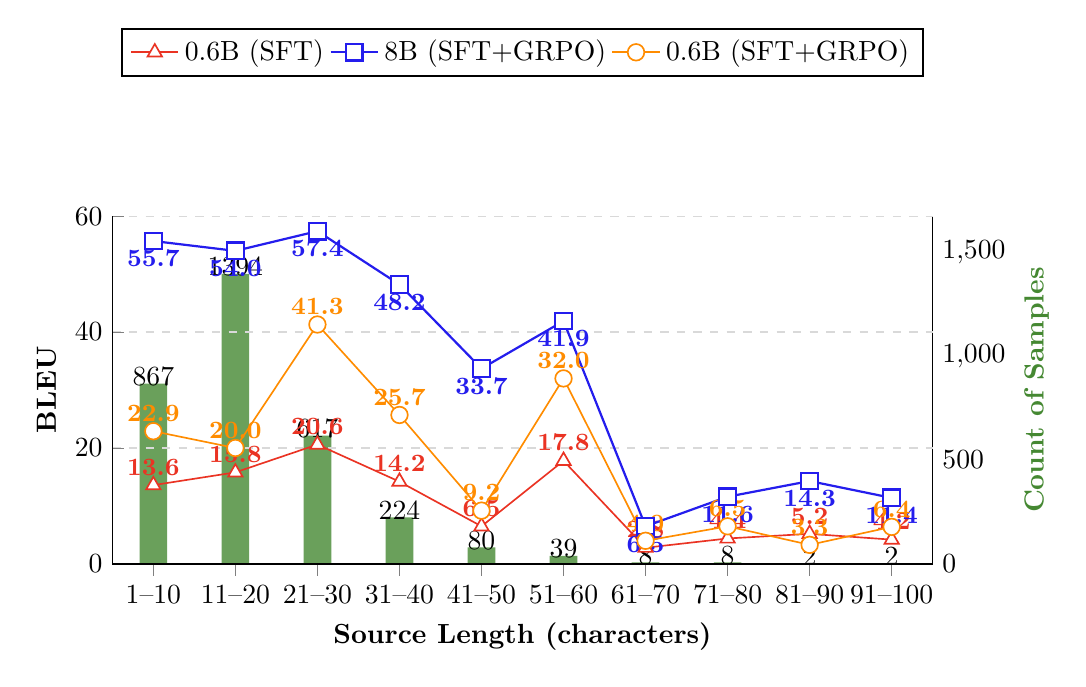
\begin{tikzpicture}[yshift=-1.5cm]
    % Bar chart (right axis) - draw first, at lower layer
    \begin{axis}[
        width=12cm, height=6cm,
        axis y line*=right,
        axis x line*=bottom,
        xlabel=\textbf{Source Length (characters)},
        ylabel=\textbf{\textcolor{myGreen}{Count of Samples}},
        ybar,
        bar width=10pt,
        xmin=0, xmax=100,
        xtick={5,15,25,35,45,55,65,75,85,95},
        xticklabels={1--10,11--20,21--30,31--40,41--50,51--60,61--70,71--80,81--90,91--100},
        ymin=0, ymax=1672,
        ytick style={draw=none},
    ]
        \addplot[
            fill=myGreen!80,
            draw=none,
        ] coordinates {
            (5,867)
            (15,1394)
            (25,617)
            (35,224)
            (45,80)
            (55,39)
            (65,8)
            (75,8)
            (85,2)
            (95,2)
        };

        \node at (axis cs:5,900) {867};
        \node at (axis cs:15,1427) {1394};
        \node at (axis cs:25,650) {617};
        \node at (axis cs:35,257) {224};
        \node at (axis cs:45,113) {80};
        \node at (axis cs:55,72) {39};
        \node at (axis cs:65,41) {8};
        \node at (axis cs:75,41) {8};
        \node at (axis cs:85,35) {2};
        \node at (axis cs:95,35) {2};

    \end{axis}

    % Line chart (left axis) - draw second, on top layer
    \begin{axis}[
        width=12cm, height=6cm,
        axis y line*=left,
        axis x line*=none,
        ylabel=\textbf{BLEU},
        xmin=0, xmax=100,
        ymin=0, ymax=60,
        xtick=\empty,
        grid=major,
        grid style={dashed, gray!30},
        clip=false,
        legend style={
            at={(0.5,1.4)},
            anchor=south,
            legend columns=3,
            draw=black,
            thick,
            fill=white,
        }
    ]
        % --- 0.6B (SFT) ---
        \addplot+[
            color=mySalmon,
            mark=triangle*,
            mark options={fill=white, scale=1.5},
            semithick,
        ] coordinates {
            (5,13.6) (15,15.8) (25,20.6) (35,14.2) (45,6.5) (55,17.8) (65,2.8) (75,4.4) (85,5.2) (95,4.2)
        };
        \addlegendentry{0.6B (SFT)}

        \node[above] at (axis cs:5,13.6) {\small\bfseries\textcolor{mySalmon}{13.6}};
        \node[above] at (axis cs:15,15.8) {\small\bfseries\textcolor{mySalmon}{15.8}};
        \node[above] at (axis cs:25,20.6) {\small\bfseries\textcolor{mySalmon}{20.6}};
        \node[above] at (axis cs:35,14.2) {\small\bfseries\textcolor{mySalmon}{14.2}};
        \node[above] at (axis cs:45,6.5) {\small\bfseries\textcolor{mySalmon}{6.5}};
        \node[above] at (axis cs:55,17.8) {\small\bfseries\textcolor{mySalmon}{17.8}};
        \node[above] at (axis cs:65,2.8) {\small\bfseries\textcolor{mySalmon}{2.8}};
        \node[above] at (axis cs:75,4.4) {\small\bfseries\textcolor{mySalmon}{4.4}};
        \node[above] at (axis cs:85,5.2) {\small\bfseries\textcolor{mySalmon}{5.2}};
        \node[above] at (axis cs:95,4.2) {\small\bfseries\textcolor{mySalmon}{4.2}};

        % --- 8B (SFT+GRPO) ---
        \addplot+[
            color=myBlue,
            mark=square*,
            mark options={fill=white, scale=1.5},
            thick,
        ] coordinates {
            (5,55.7) (15,54.0) (25,57.4) (35,48.2) (45,33.7) (55,41.9) (65,6.5) (75,11.6) (85,14.3) (95,11.4)
        };
        \addlegendentry{8B (SFT+GRPO)}

        \node[below] at (axis cs:5,55.7) {\small\bfseries\textcolor{myBlue}{55.7}};
        \node[below] at (axis cs:15,54.0) {\small\bfseries\textcolor{myBlue}{54.0}};
        \node[below] at (axis cs:25,57.4) {\small\bfseries\textcolor{myBlue}{57.4}};
        \node[below] at (axis cs:35,48.2) {\small\bfseries\textcolor{myBlue}{48.2}};
        \node[below] at (axis cs:45,33.7) {\small\bfseries\textcolor{myBlue}{33.7}};
        \node[below] at (axis cs:55,41.9) {\small\bfseries\textcolor{myBlue}{41.9}};
        \node[below] at (axis cs:65,6.5) {\small\bfseries\textcolor{myBlue}{6.5}};
        \node[below] at (axis cs:75,11.6) {\small\bfseries\textcolor{myBlue}{11.6}};
        \node[below] at (axis cs:85,14.3) {\small\bfseries\textcolor{myBlue}{14.3}};
        \node[below] at (axis cs:95,11.4) {\small\bfseries\textcolor{myBlue}{11.4}};

        % --- 0.6B (SFT+GRPO) ---
        \addplot+[
            color=myOrange,
            mark=*,
            mark options={fill=white, scale=1.5},
            semithick,
        ] coordinates {
            (5,22.9) (15,20.0) (25,41.3) (35,25.7) (45,9.2) (55,32.0) (65,4.0) (75,6.5) (85,3.3) (95,6.4)
        };
        \addlegendentry{0.6B (SFT+GRPO)}

        \node[above] at (axis cs:5,22.9) {\small\bfseries\textcolor{myOrange}{22.9}};
        \node[above] at (axis cs:15,20.0) {\small\bfseries\textcolor{myOrange}{20.0}};
        \node[above] at (axis cs:25,41.3) {\small\bfseries\textcolor{myOrange}{41.3}};
        \node[above] at (axis cs:35,25.7) {\small\bfseries\textcolor{myOrange}{25.7}};
        \node[above] at (axis cs:45,9.2) {\small\bfseries\textcolor{myOrange}{9.2}};
        \node[above] at (axis cs:55,32.0) {\small\bfseries\textcolor{myOrange}{32.0}};
        \node[above] at (axis cs:65,4.0) {\small\bfseries\textcolor{myOrange}{4.0}};
        \node[above] at (axis cs:75,6.5) {\small\bfseries\textcolor{myOrange}{6.5}};
        \node[above] at (axis cs:85,3.3) {\small\bfseries\textcolor{myOrange}{3.3}};
        \node[above] at (axis cs:95,6.4) {\small\bfseries\textcolor{myOrange}{6.4}};

    \end{axis}
\end{tikzpicture}

\end{document}
